\section{ITSA-58-3 完整二元樹}
\centerline{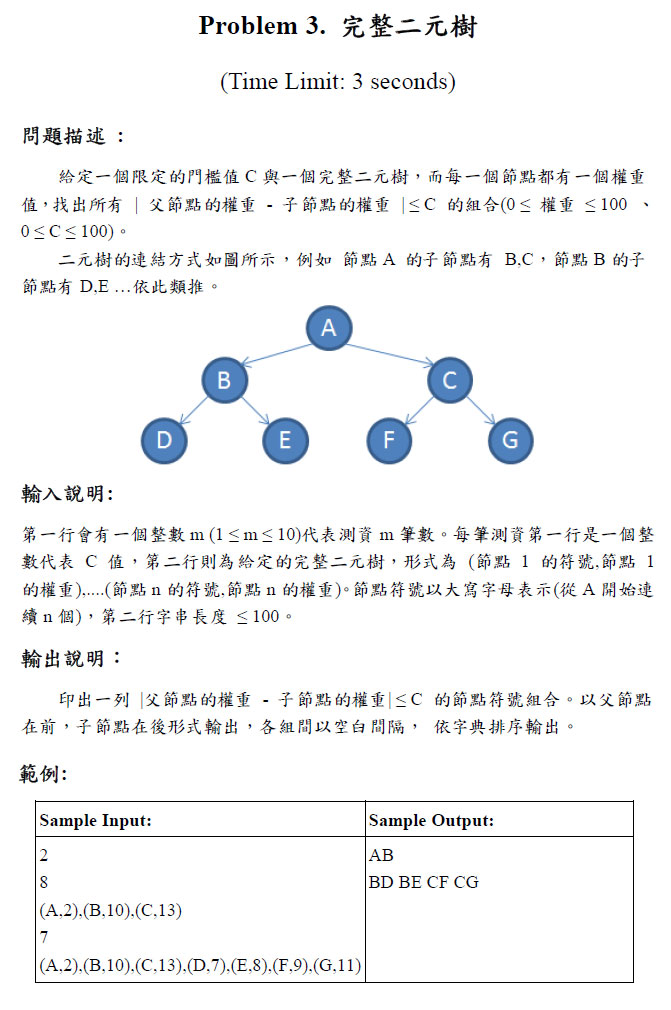
\includegraphics[height=.95\textheight]{../solutions/fig/58ITSA3}}

\subsection{解題思惟}
\begin{enumerate}
	\item $n$層的完整二元樹的節點總共有$2^n-1$個。如果我們從最上層依次從1往下編號的話,仔細檢查,會發現節點$n$的子節點分別是$2n$和$2n+1$。
	\item 讀入的資料,ABC...是依照順序來的,那節點編號也是依次來的,所以其實ABC這些字元可以不用管它,因為節點$i$對應的字元會是'A'+$i-1=64+i$。
	\item 所以我們只要能夠依次讀入$2^n-1$個權重數字到陣列就可以了,假設權重陣列為treeW,接著就是檢查父節點和兩個子節點的權重差距是否在設定的範圍之內,也就是treeW[i]和treeW[2*i]的差以及treeW[i]和treeW[2*i+1]的差是否小於等於C。
	\item 讀入資料的部份怎麼處理呢?首先,每一個case會有幾個節點是不知道的,給定的格式就是用換行結尾的,那如果我們依次讀取字元,等檢查到換行符號的時候,就表示這個case所有的資料都讀完了。要注意的是,如果我們使用scanf來讀取字元,那麼換行符號也會讀到,但如果使用\cc{}來讀取字元,預設的狀況是會忽略空白類的字元,所以會讀不到換行字元,如果要在\cc{}裡面讀到空白字元的話,要先使用以下指令,告訴編譯器不要忽略空白:
	\begin{inside}
		cin >> noskipws;
	\end{inside}
	反之,如果要回到預設忽略空白的情況,則使用以下指令:
	\begin{inside}
		cin >> skipws;
	\end{inside}
	\item 每一組資料都是從左括號開始,如果沒有碰到左括號,我們可以一直讀取字元並把它忽略,讀到左括號之後,後面就是節點字元和它的權重了。接下來我們看一下資料格式,數字一定是在「,」之後,那我們可以繼續一直讀取字元,直到出現「,」為止,碰到「,」之後,接下來就可以直接讀進一個權重數字。
\end{enumerate}
\subsection{程式碼}
\begin{cppcode}
#include <iostream>

using namespace std;

int main()
{
	int kase, C, treeW[105];
	char ch;
	cin >> kase;
	while (kase--) {
		cin >> C;
		int index = 1;
		cin >> skipws; // 一開始不會是換行字元,先忽略空白
		while ((cin>>ch) && (ch!='\n')) { // 進字元迴圈後,以換行結束
			cin >> noskipws; // 進字元迴圈後,不能忽略空白
			if (ch!='(') continue; // 不是左括號,回上面繼續讀
			while ((cin>>ch) && (ch!=',')) ; // 一直讀到「,」為止
			cin >> treeW[index++]; // 讀進權重
		}
		bool first = true; // 這是用來處理輸出各組間空白用的
		for (int p=1; p<index/2; p++) {
			for (int child=2*p; child<2*p+2; child++) {
				int diff = treeW[p] - treeW[child];
				if (diff>=-C && diff<=C) { // 差的絕對值<=C
					if (first) first = false;
					else cout << " "; // 不是第一組的話,先印空白
					cout << (char)(64+p) << (char)(64+child);
				}
			}
		}
		cout << endl;
	}
	return 0;
}
\end{cppcode}